\documentclass{beamer}
\usepackage{geometry}
\usepackage[T1]{fontenc}
%\usepackage{graphicx}
\usepackage{hyperref}
\usepackage{datetime}
\usepackage{booktabs}
\usepackage{listings}

\usepackage{tikz}
\usepackage{keyval}
\usepackage{ifthen}

\usepackage[figwidth=8cm]{todonotes}

\usepackage[british]{babel}

\usetheme{metropolis}

\title{Generate 3D models for large-scale objects}
\author{Jaan Toots \and Viorica Patraucean}
\institute[CSIC]{Cambridge Centre for Smart Infrastructure and
  Construction}
\date{\formatdate{24}{10}{2016}}

\begin{document}

\maketitle

\section{Approach}

\begin{frame}{Deep learning for semantic and geometric segmentation}
  \begin{figure}[h]\centering
    \only<1>{\includegraphics[width=9cm]{ninewells-photo.jpg}}
    \only<2>{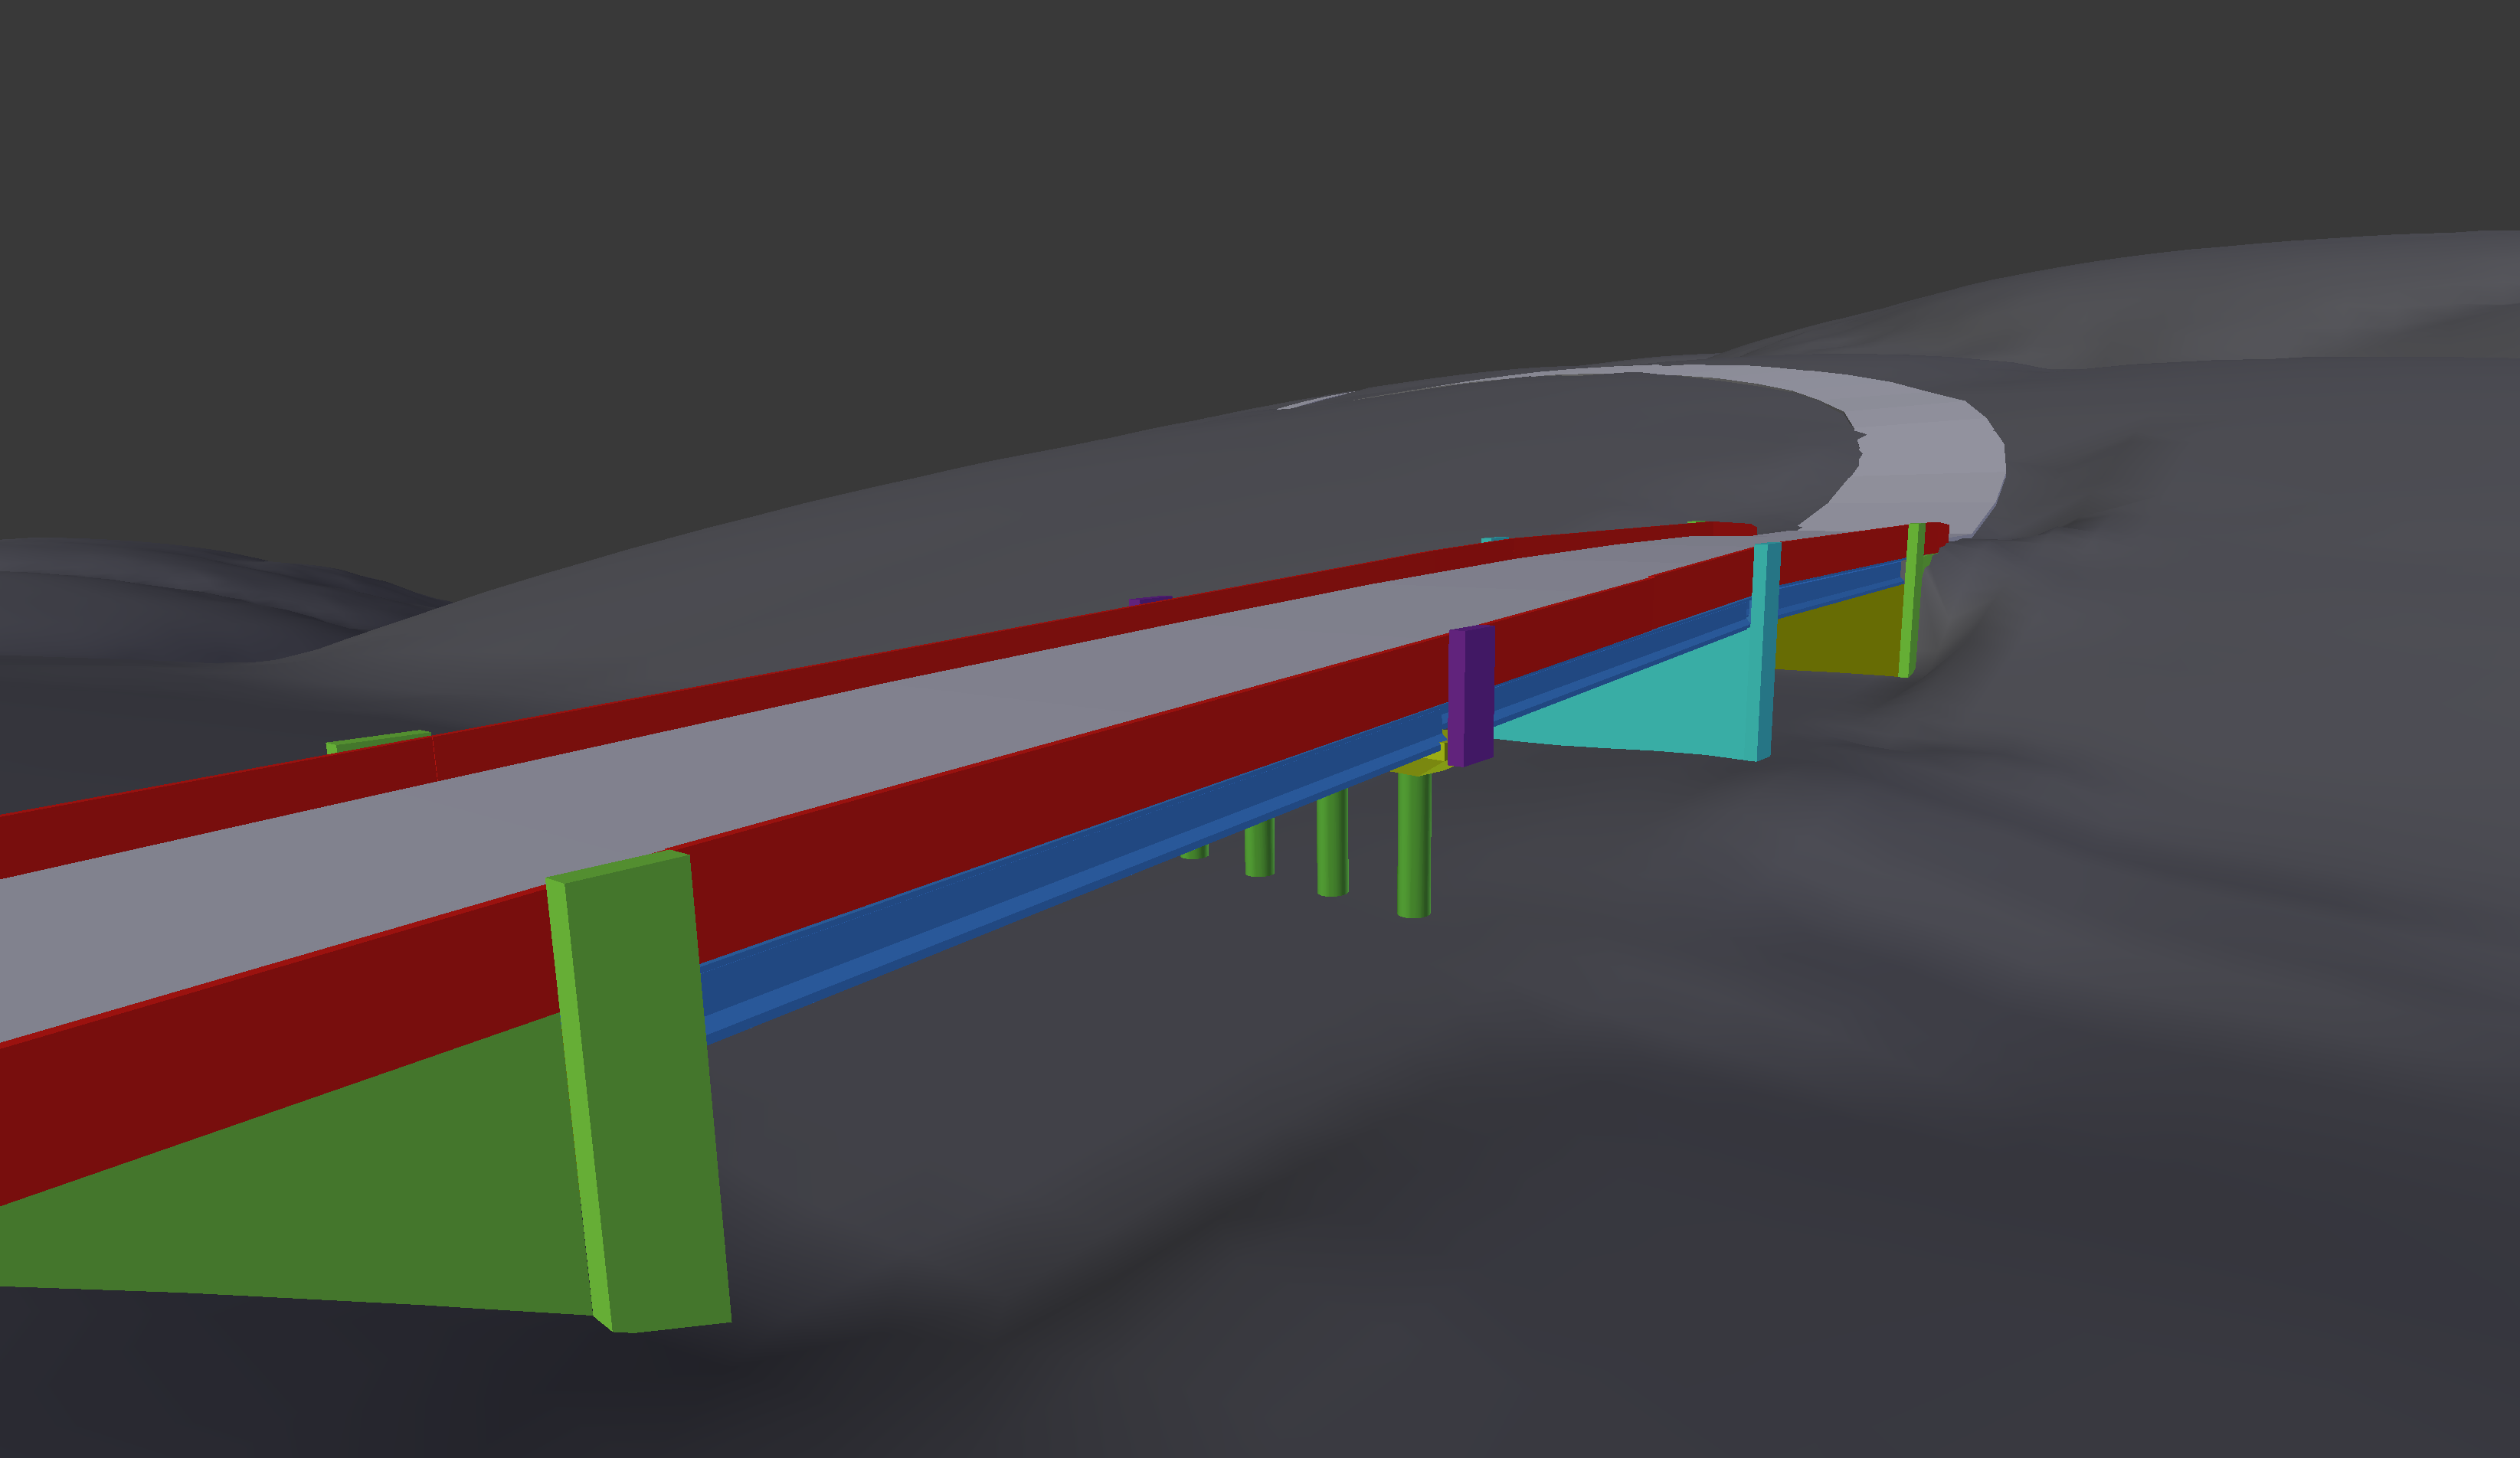
\includegraphics[width=9cm]{ninewells-view.png}}
  \end{figure}
  
\end{frame}
\note{The project aims at generating BIM (Building Information Model)
  for existing bridges in an automatic way. This requires modelling
  the geometry and the materials of the bridge components. Material
  recognition from images is (relatively) solved. The challenge is on
  the geometry side.}
\note{\ldots which amounts to recognising for each bridge part what it
  represents and what shape it has, e.g.\ a column that has
  cylindrical shape. Once this info is available, a geometric fitting
  step is needed to get the parameters for each part. Due to the
  recent success of deep learning in various tasks like image
  labelling, object detection, semantic segmentation, we decided to
  use a deep learning based approach as well.}

\begin{frame}{Neural networks}
  \begin{figure}[h]\centering
    \def\layersep{2cm}

\begin{tikzpicture}[shorten >=1pt,->,draw=black!50, node distance=\layersep]
  \tikzstyle{every pin edge}=[shorten <=1pt]
  \tikzstyle{neuron}=[circle,fill=black!25,minimum size=17pt,inner sep=0pt]
  \tikzstyle{input neuron}=[neuron, fill=green!50];
  \tikzstyle{output neuron}=[neuron, fill=red!50];
  \tikzstyle{hidden neuron}=[neuron, fill=blue!50];
  \tikzstyle{annot} = [text width=4em, text centered]

  % Draw the input layer nodes
  \foreach \name / \y in {1,...,3}
  % This is the same as writing \foreach \name / \y in {1/1,2/2,3/3,4/4}
  \node[input neuron, pin={[pin edge={<-}]left:}] (I-\name) at (0,-\y) {};

  \node[annot, above of=I-1, node distance=1cm] (il) {\scriptsize input layer};

  % Draw the hidden layer nodes
  \foreach \name / \y in {1,...,4} \path[yshift=0.5cm] node[hidden
  neuron] (H1-\name) at (\layersep,-\y cm) {};

  \node[annot, above of=H1-1, node distance=1cm] (h1l) {\scriptsize hidden layer 1};
  
  \foreach \name / \y in {1,...,4} \path[yshift=0.5cm] node[hidden
  neuron] (H2-\name) at (2*\layersep,-\y cm) {};

  \node[annot, above of=H2-1, node distance=1cm] (h2l) {\scriptsize hidden layer 2};

  \foreach \name / \y in {1,...,4} \path[yshift=0.5cm] node[hidden
  neuron] (H3-\name) at (3*\layersep,-\y cm) {};

  \node[annot, above of=H3-1, node distance=1cm] (h3l) {\scriptsize hidden layer 3};

  % Draw the output layer node
  \foreach \name / \y in {1,...,2} \path[yshift=-0.5cm] node[output
  neuron, pin={[pin edge={->}]right:}] (O-\name) at
  (4*\layersep,-\y cm) {};

  \node[annot, above of=O-1, node distance=1cm] (ol) {\scriptsize output layer};

  % Connect nodes
  \foreach \source in {1,...,3}
  \foreach \dest in {1,...,4}
  \path (I-\source) edge (H1-\dest);

  \foreach \source in {1,...,4}
  \foreach \dest in {1,...,4}
  \path (H1-\source) edge (H2-\dest);

  \foreach \source in {1,...,4}
  \foreach \dest in {1,...,4}
  \path (H2-\source) edge (H3-\dest);

  \foreach \source in {1,...,4}
  \foreach \dest in {1,...,2}
  \path (H3-\source) edge (O-\dest);
\end{tikzpicture}

  \end{figure}
\end{frame}
\note{Deep learning relies on deep neural networks, which are powerful
  models, with high capacity to learn from examples. But large
  training sets are required because the models can have millions of
  parameters. Moreover, training a neural network requires high
  computational resources. Existing methods deal mainly with text,
  images, or videos, and existing computational resources (GPUs) can
  accommodate them.}
\note{For our problem, we would prefer images and videos, but methods
  for estimating depth and 3D from images are not sufficiently
  accurate. So we need to use point clouds, which provide accurate
  geometry. But point clouds contain millions of 3D points, having
  huge memory requirements, and cannot be used efficiently for GPU
  processing.}

\subsection{Input}

\begin{frame}{Unordered point-cloud}
  \begin{figure}[h]\centering
    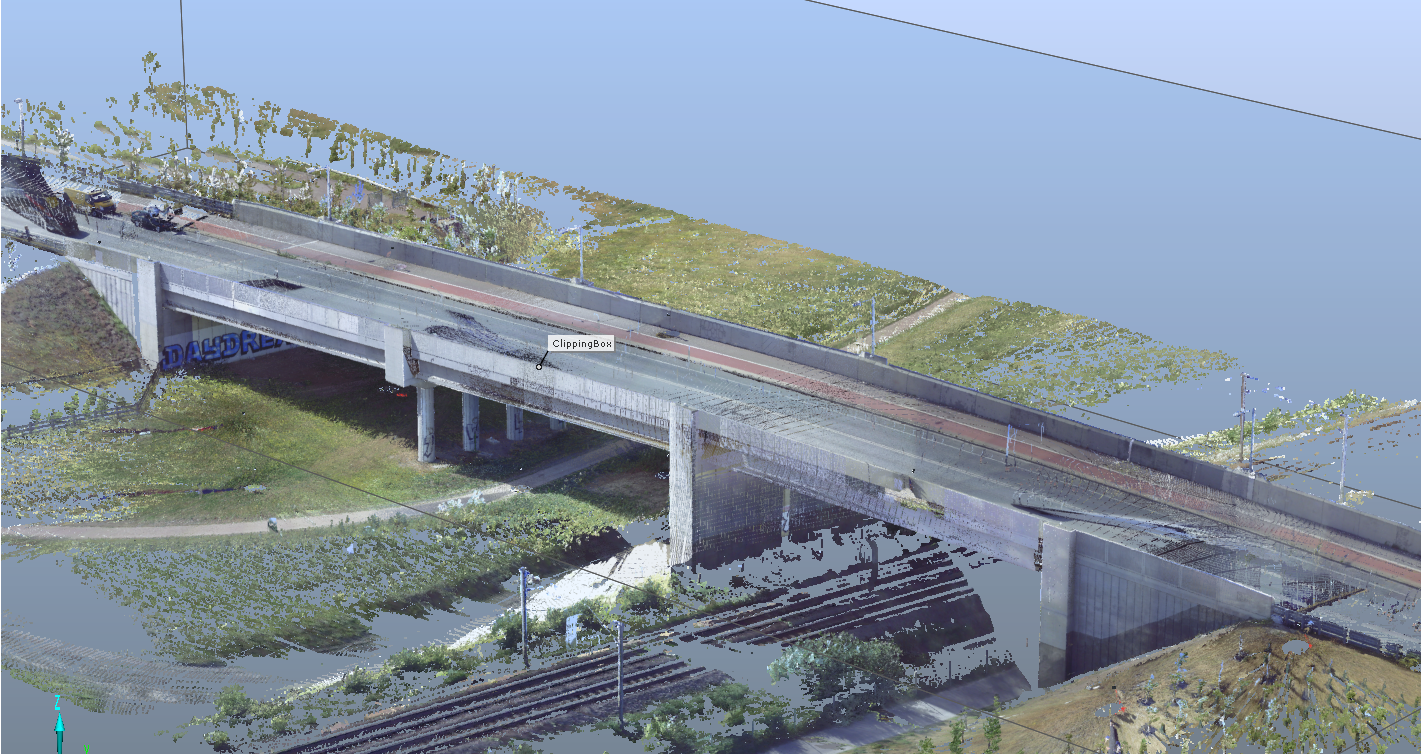
\includegraphics[width=9cm]{ninewells-cloud.png}
  \end{figure}
\end{frame}
\note{This is because we need to deal with unordered point clouds,
  like the ones the laser-scanners provide after registration. An
  unordered point cloud is a set of points with 3D coordinates. This
  is opposed to ordered point-clouds, e.g.\ occupancy grids or depth
  maps.}

\begin{frame}{Occupancy grid}
  \begin{figure}[h]\centering
    % Based on [TeX Stack Exchange answer](http://tex.stackexchange.com/a/29882)
% by [Tom Bombadil](http://tex.stackexchange.com/users/7279/tom-bombadil)
% CC BY-SA 3.0

\makeatletter
% Standard Values for Parameters
\newcommand{\tikzcuboid@shiftx}{0}
\newcommand{\tikzcuboid@shifty}{0}
\newcommand{\tikzcuboid@dimx}{4}
\newcommand{\tikzcuboid@dimy}{4}
\newcommand{\tikzcuboid@dimz}{4}
\newcommand{\tikzcuboid@scale}{1}
\newcommand{\tikzcuboid@densityx}{1}
\newcommand{\tikzcuboid@densityy}{1}
\newcommand{\tikzcuboid@densityz}{1}
\newcommand{\tikzcuboid@rotation}{0}
\newcommand{\tikzcuboid@anglex}{0}
\newcommand{\tikzcuboid@angley}{90}
\newcommand{\tikzcuboid@anglez}{225}
\newcommand{\tikzcuboid@scalex}{1}
\newcommand{\tikzcuboid@scaley}{1}
\newcommand{\tikzcuboid@scalez}{1}
\newcommand{\tikzcuboid@linefront}{}
\newcommand{\tikzcuboid@linetop}{}
\newcommand{\tikzcuboid@lineright}{}
\newcommand{\tikzcuboid@fillfront}{}
\newcommand{\tikzcuboid@filltop}{}
\newcommand{\tikzcuboid@fillright}{}
\newcommand{\tikzcuboid@newcoords}{N}
\newcommand{\tikzcuboid@filled}{N}
\newcommand{\tikzcuboid@shaded}{N}
% Definition of Keys
\define@key{tikzcuboid}{shiftx}[\tikzcuboid@shiftx]{\renewcommand{\tikzcuboid@shiftx}{#1}}
\define@key{tikzcuboid}{shifty}[\tikzcuboid@shifty]{\renewcommand{\tikzcuboid@shifty}{#1}}
\define@key{tikzcuboid}{dimx}[\tikzcuboid@dimx]{\renewcommand{\tikzcuboid@dimx}{#1}}
\define@key{tikzcuboid}{dimy}[\tikzcuboid@dimy]{\renewcommand{\tikzcuboid@dimy}{#1}}
\define@key{tikzcuboid}{dimz}[\tikzcuboid@dimz]{\renewcommand{\tikzcuboid@dimz}{#1}}
\define@key{tikzcuboid}{scale}[\tikzcuboid@scale]{\renewcommand{\tikzcuboid@scale}{#1}}
\define@key{tikzcuboid}{densityx}[\tikzcuboid@densityx]{\renewcommand{\tikzcuboid@densityx}{#1}}
\define@key{tikzcuboid}{densityy}[\tikzcuboid@densityy]{\renewcommand{\tikzcuboid@densityy}{#1}}
\define@key{tikzcuboid}{densityz}[\tikzcuboid@densityz]{\renewcommand{\tikzcuboid@densityz}{#1}}
\define@key{tikzcuboid}{rotation}[\tikzcuboid@rotation]{\renewcommand{\tikzcuboid@rotation}{#1}}
\define@key{tikzcuboid}{anglex}[\tikzcuboid@anglex]{\renewcommand{\tikzcuboid@anglex}{#1}}
\define@key{tikzcuboid}{angley}[\tikzcuboid@angley]{\renewcommand{\tikzcuboid@angley}{#1}}
\define@key{tikzcuboid}{anglez}[\tikzcuboid@anglez]{\renewcommand{\tikzcuboid@anglez}{#1}}
\define@key{tikzcuboid}{scalex}[\tikzcuboid@scalex]{\renewcommand{\tikzcuboid@scalex}{#1}}
\define@key{tikzcuboid}{scaley}[\tikzcuboid@scaley]{\renewcommand{\tikzcuboid@scaley}{#1}}
\define@key{tikzcuboid}{scalez}[\tikzcuboid@scalez]{\renewcommand{\tikzcuboid@scalez}{#1}}
\define@key{tikzcuboid}{linefront}[\tikzcuboid@linefront]{\renewcommand{\tikzcuboid@linefront}{#1}}
\define@key{tikzcuboid}{linetop}[\tikzcuboid@linetop]{\renewcommand{\tikzcuboid@linetop}{#1}}
\define@key{tikzcuboid}{lineright}[\tikzcuboid@lineright]{\renewcommand{\tikzcuboid@lineright}{#1}}
\define@key{tikzcuboid}{fillfront}[\tikzcuboid@fillfront]{\renewcommand{\tikzcuboid@fillfront}{#1}}
\define@key{tikzcuboid}{filltop}[\tikzcuboid@filltop]{\renewcommand{\tikzcuboid@filltop}{#1}}
\define@key{tikzcuboid}{fillright}[\tikzcuboid@fillright]{\renewcommand{\tikzcuboid@fillright}{#1}}
\define@key{tikzcuboid}{newcoords}[\tikzcuboid@newcoords]{\renewcommand{\tikzcuboid@newcoords}{#1}}
\define@key{tikzcuboid}{filled}[\tikzcuboid@filled]{\renewcommand{\tikzcuboid@filled}{#1}}
\define@key{tikzcuboid}{shaded}[\tikzcuboid@shaded]{\renewcommand{\tikzcuboid@shaded}{#1}}
% Commands
\newcommand{\tikzcuboid}[1]{
    \setkeys{tikzcuboid}{#1} % Process Keys passed to command
    \begin{scope}[xshift=\tikzcuboid@shiftx,yshift=\tikzcuboid@shifty,scale=\tikzcuboid@scale,rotate=\tikzcuboid@rotation]
    \pgfmathsetmacro{\steppingx}{1/\tikzcuboid@densityx}
    \pgfmathsetmacro{\steppingy}{1/\tikzcuboid@densityy}
    \pgfmathsetmacro{\steppingz}{1/\tikzcuboid@densityz}
    \newcommand{\dimx}{\tikzcuboid@dimx}
    \newcommand{\dimy}{\tikzcuboid@dimy}
    \newcommand{\dimz}{\tikzcuboid@dimz}
    \pgfmathsetmacro{\secondx}{2*\steppingx}
    \pgfmathsetmacro{\secondy}{2*\steppingy}
    \pgfmathsetmacro{\secondz}{2*\steppingz}
    \foreach \x in {\steppingx,\secondx,...,\dimx}
    {   \foreach \y in {\steppingy,\secondy,...,\dimy}
        {   \pgfmathsetmacro{\lowx}{(\x-\steppingx)}
            \pgfmathsetmacro{\lowy}{(\y-\steppingy)}
            \draw (\lowx,\lowy,\dimz) -- (\lowx,\y,\dimz) -- (\x,\y,\dimz) -- (\x,\lowy,\dimz) -- cycle;

        }
    }
    \foreach \x in {\steppingx,\secondx,...,\dimx}
    {   \foreach \z in {\steppingz,\secondz,...,\dimz}
        {   \pgfmathsetmacro{\lowx}{(\x-\steppingx)}
            \pgfmathsetmacro{\lowz}{(\z-\steppingz)}
            \draw (\lowx,\dimy,\lowz) -- (\lowx,\dimy,\z) -- (\x,\dimy,\z) -- (\x,\dimy,\lowz) -- cycle;
        }
    }
    \foreach \y in {\steppingy,\secondy,...,\dimy}
    {   \foreach \z in {\steppingz,\secondz,...,\dimz}
        {   \pgfmathsetmacro{\lowy}{(\y-\steppingy)}
            \pgfmathsetmacro{\lowz}{(\z-\steppingz)}
            \draw (\dimx,\lowy,\lowz) -- (\dimx,\lowy,\z) -- (\dimx,\y,\z) -- (\dimx,\y,\lowz) -- cycle;
        }
    }
    \end{scope}

    % Write parameters to log file, just for checking       
%   \typeout{=============================}
%   \typeout{*****************************}
%   \typeout{tikzcuboid shiftx = \tikzcuboid@shiftx}
%   \typeout{tikzcuboid shifty = \tikzcuboid@shifty}
%   \typeout{tikzcuboid dimx = \tikzcuboid@dimx}
%   \typeout{tikzcuboid dimy = \tikzcuboid@dimy}
%   \typeout{tikzcuboid dimz = \tikzcuboid@dimz}
%   \typeout{tikzcuboid scale = \tikzcuboid@scale}
%   \typeout{tikzcuboid densityx = \tikzcuboid@densityx}
%   \typeout{tikzcuboid densityy = \tikzcuboid@densityy}
%   \typeout{tikzcuboid densityz = \tikzcuboid@densityz}
%   \typeout{tikzcuboid rotation = \tikzcuboid@rotation}
%   \typeout{tikzcuboid anglex = \tikzcuboid@anglex}
%   \typeout{tikzcuboid angley = \tikzcuboid@angley}
%   \typeout{tikzcuboid anglez = \tikzcuboid@anglez}
%   \typeout{tikzcuboid scalex = \tikzcuboid@scalex}
%   \typeout{tikzcuboid scaley = \tikzcuboid@scaley}
%   \typeout{tikzcuboid scalez = \tikzcuboid@scalez}
%   \typeout{tikzcuboid linefront = \tikzcuboid@linefront}
%   \typeout{tikzcuboid linetop = \tikzcuboid@linetop}
%   \typeout{tikzcuboid lineright = \tikzcuboid@lineright}
%   \typeout{tikzcuboid fillfront = \tikzcuboid@fillfront}
%   \typeout{tikzcuboid filltop = \tikzcuboid@filltop}
%   \typeout{tikzcuboid fillright = \tikzcuboid@fillright}
%   \typeout{tikzcuboid newcoords = \tikzcuboid@newcoords}
%   \typeout{tikzcuboid filled = \tikzcuboid@filled}
%   \typeout{tikzcuboid shaded = \tikzcuboid@shaded}
%   \typeout{*****************************}
%   \typeout{=============================}
}

\makeatother

\begin{tikzpicture}
    \tikzcuboid{shiftx=0cm,%
        shifty=0cm,%
        scale=0.90,%
        rotation=0,%
        densityx=1,%
        densityy=1,%
        densityz=1%
    }
\end{tikzpicture}

  \end{figure}
\end{frame}
\note{An occupancy grid is a 3D grid where each cell is marked
  ``occupied'' if there is a point inside or ``free'' otherwise. Most
  of existing deep learning approaches for 3D point-clouds use this
  representation with 3D (volumetric) neural networks. But they work
  only with small objects (chairs, tables). The requirements for large
  structures like bridges would be prohibitive. Moreover, the memory
  would be wasted since in our case most of the cells would be marked
  as ``free''.}

\begin{frame}{Depth map}
  \begin{figure}[h]\centering
    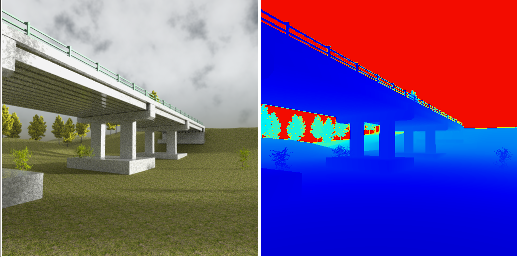
\includegraphics[width=8cm]{depth.png}
  \end{figure}
\end{frame}
\note{So we chose to represent a point cloud through RGBD images,
  without any loss of information. A depth map is an image where each
  pixel encodes the distance between the camera and the 3D points;
  here colour-coded: cold colours represent shorter distances.}

\subsection{Segmentation of bridges}

\begin{frame}{Segmentation of bridges}
  Main steps:
  \begin{itemize}
  \item Render RGB and depth images
  \item Segmentation of images
  \item Back-project labels into point-cloud
  \end{itemize}
  Because real data is difficult to obtain, we use synthetically
  textured bridge models.
\end{frame}

\section{Dataset}

\begin{frame}{Overview}
  \begin{itemize}
  \item 30 models of bridges
  \item 4535 rendered RGBD images
    \begin{itemize}
    \item 4100 training
    \item 435 test
    \end{itemize}
  \item Hierarchical labels
    \begin{itemize}
    \item Geometric labels (12)
    \item Class labels (7)
    \item Part labels (28)
    \end{itemize}
  \end{itemize}
\end{frame}

\subsection{Models}

\begin{frame}{Models}
  Start with models from various sources and prepare for
  rendering. Add landscape, roads and vegetation.

  \begin{figure}[h]\centering
    \begin{tikzpicture}
  [var/.style={circle},
    lab/.style={rectangle,fill=p-box},
    pre/.style={<-,shorten <=1pt,semithick,draw},
    post/.style={->,shorten >=1pt,semithick,draw}]
  
%  \clip (1.5,-2.5) rectangle (14.5,4.5);

  \node (aws) at (0,0) {%
    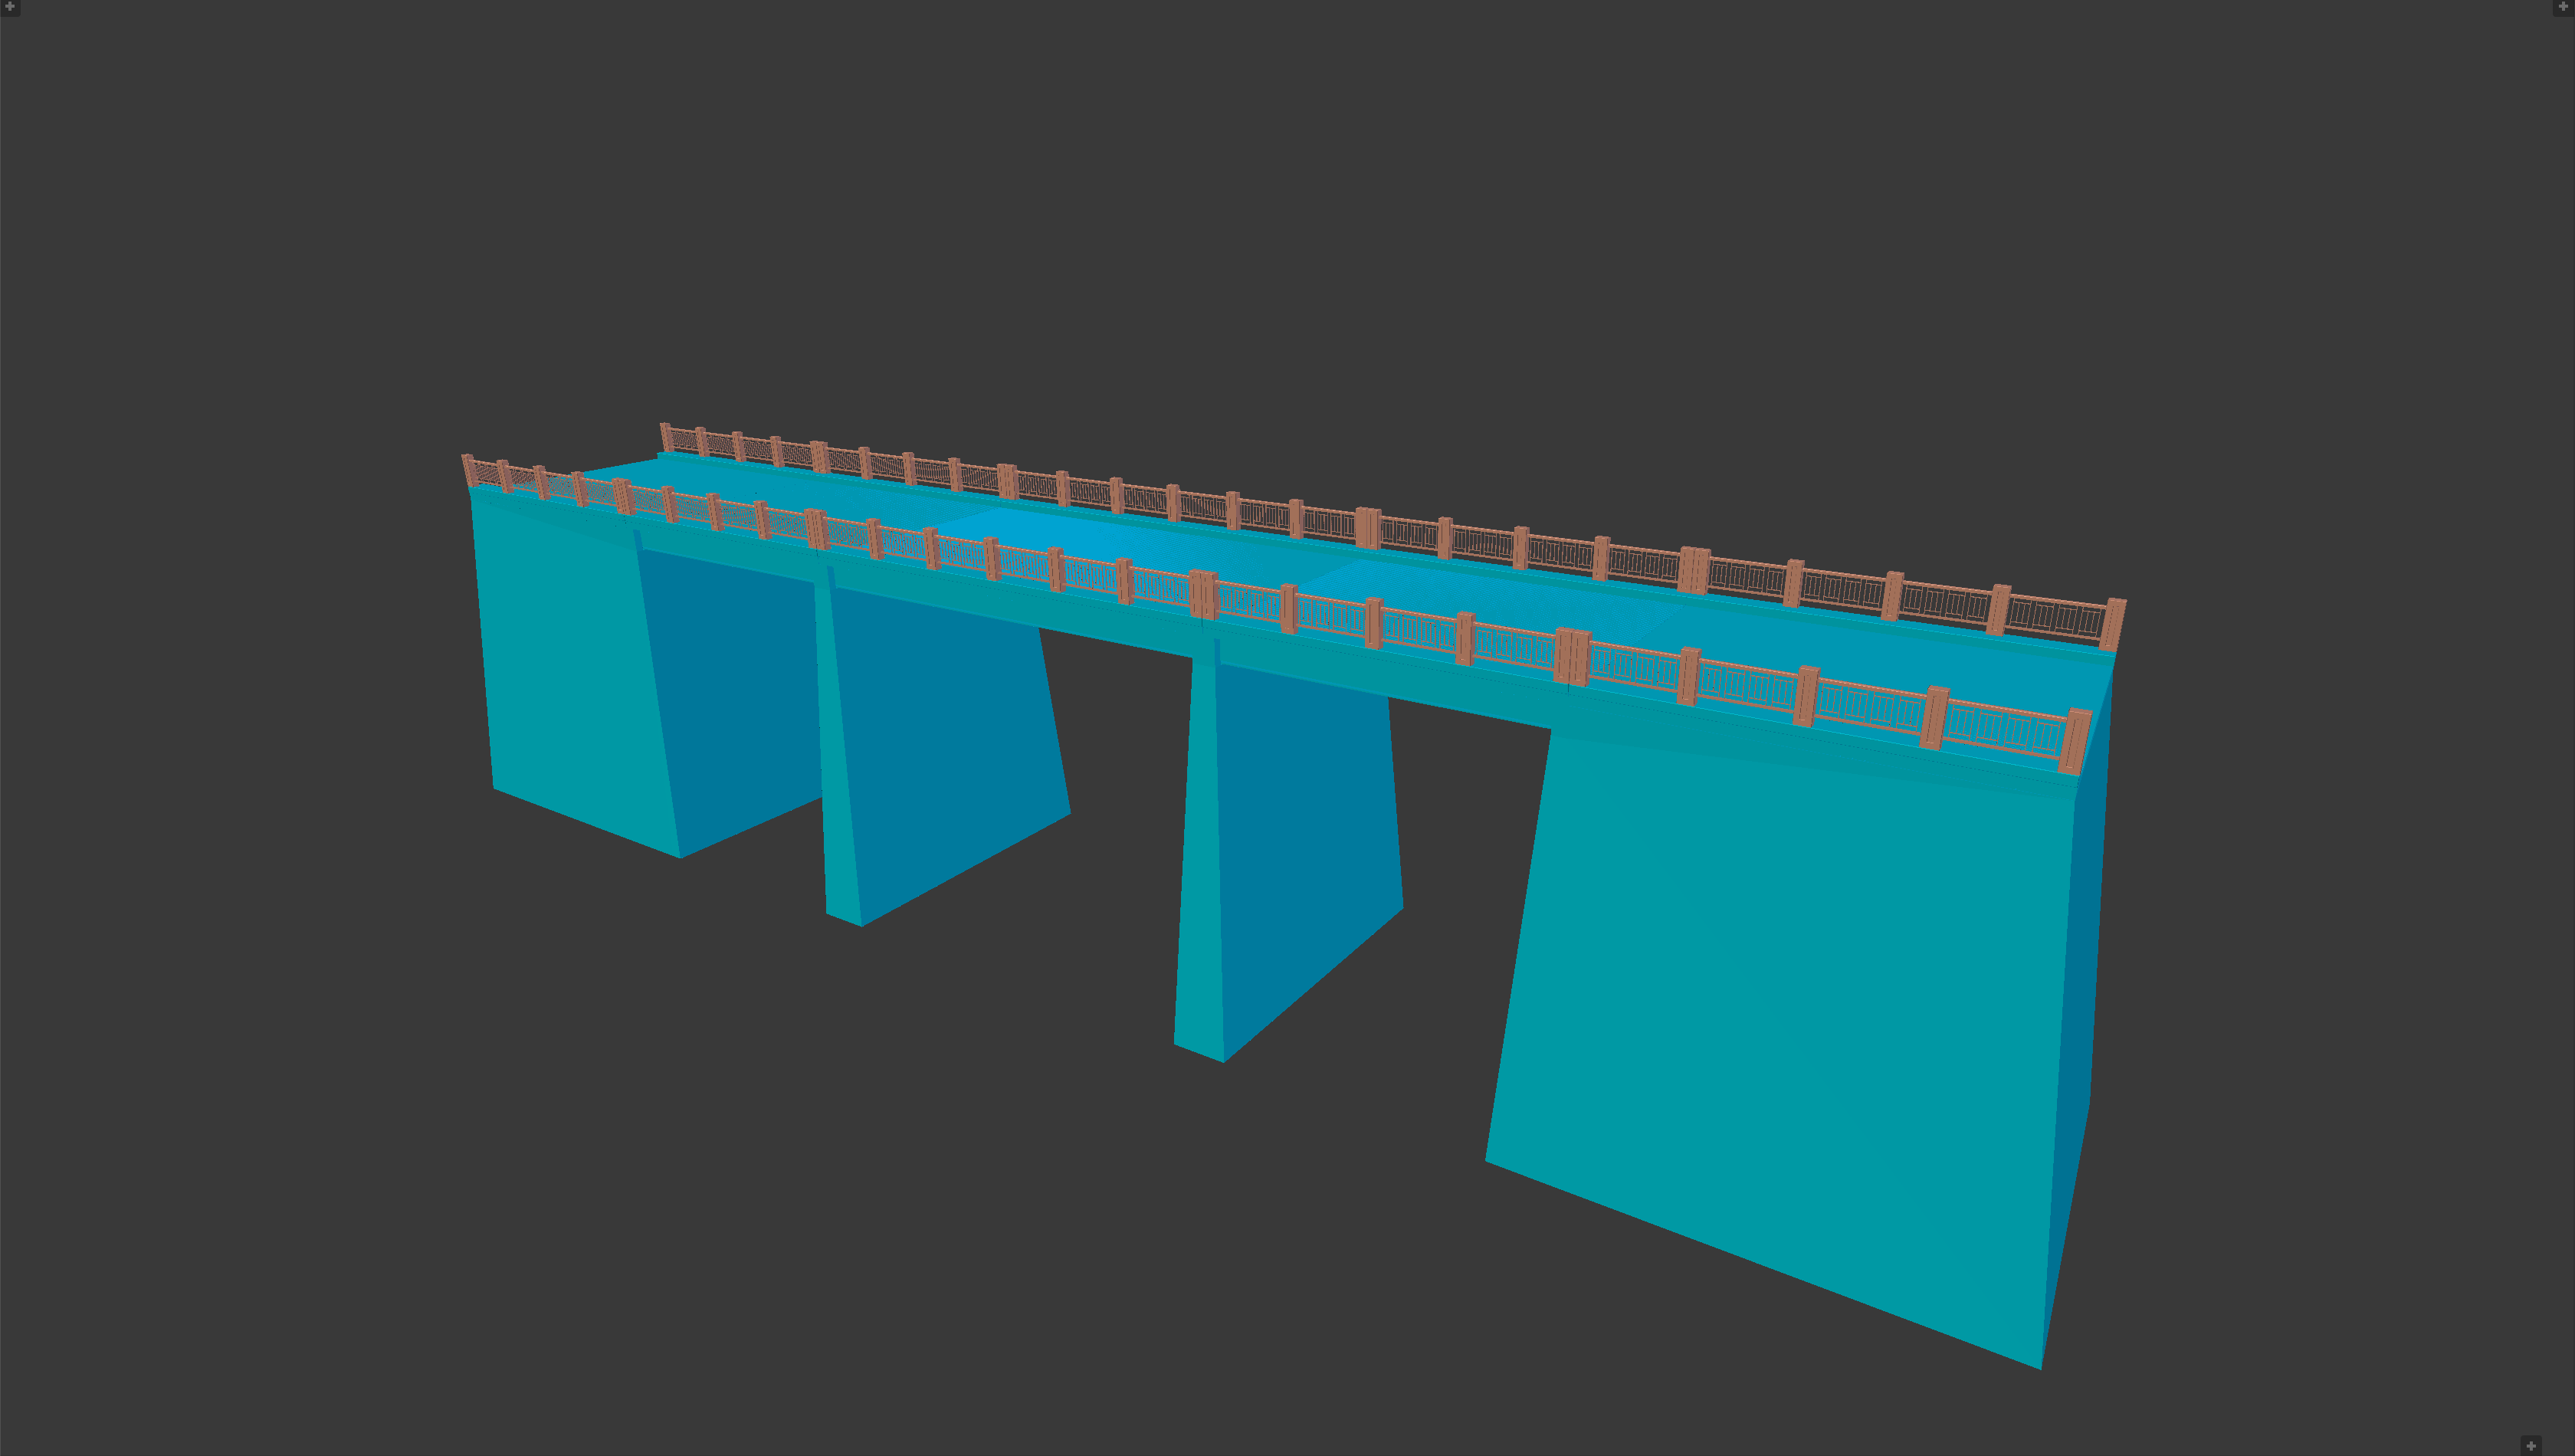
\includegraphics[width=4.5cm]{aw-start.png}
  };
  \node (awf) at (6,0) {%
    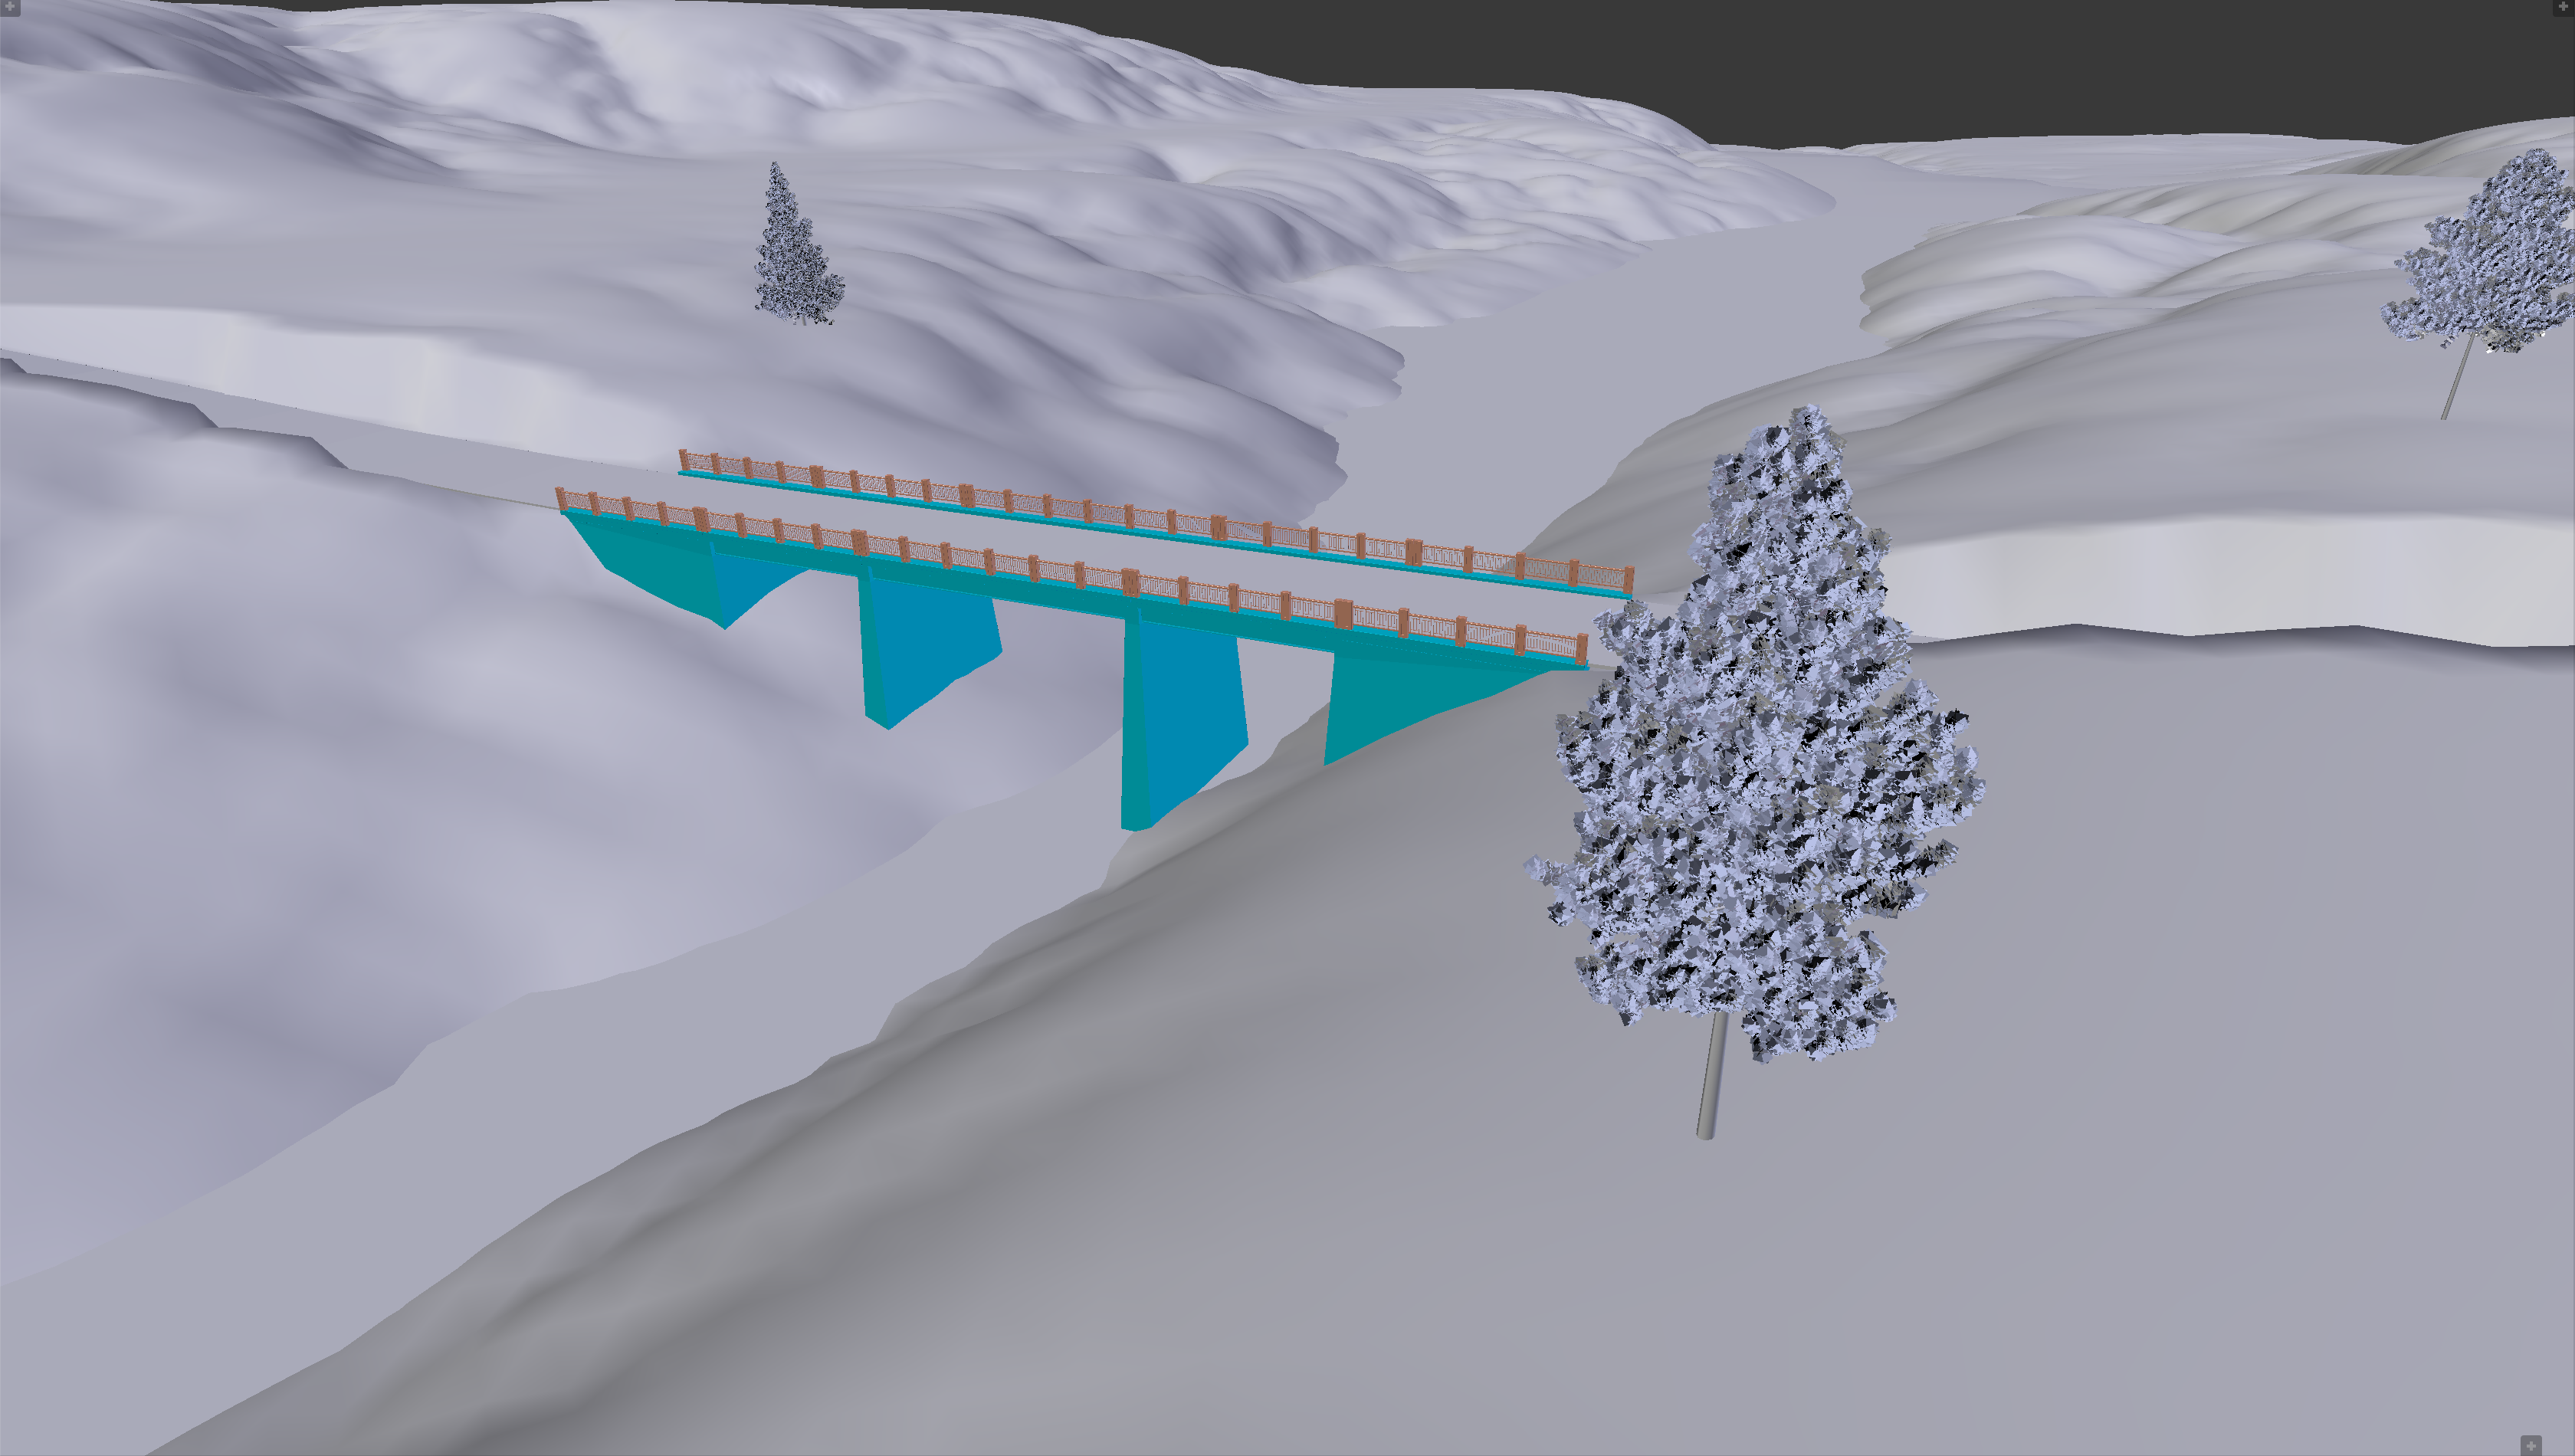
\includegraphics[width=4.5cm]{aw-final.png}
  }
  edge[pre] (aws);
\end{tikzpicture}

  \end{figure}
\end{frame}

\begin{frame}[plain]
  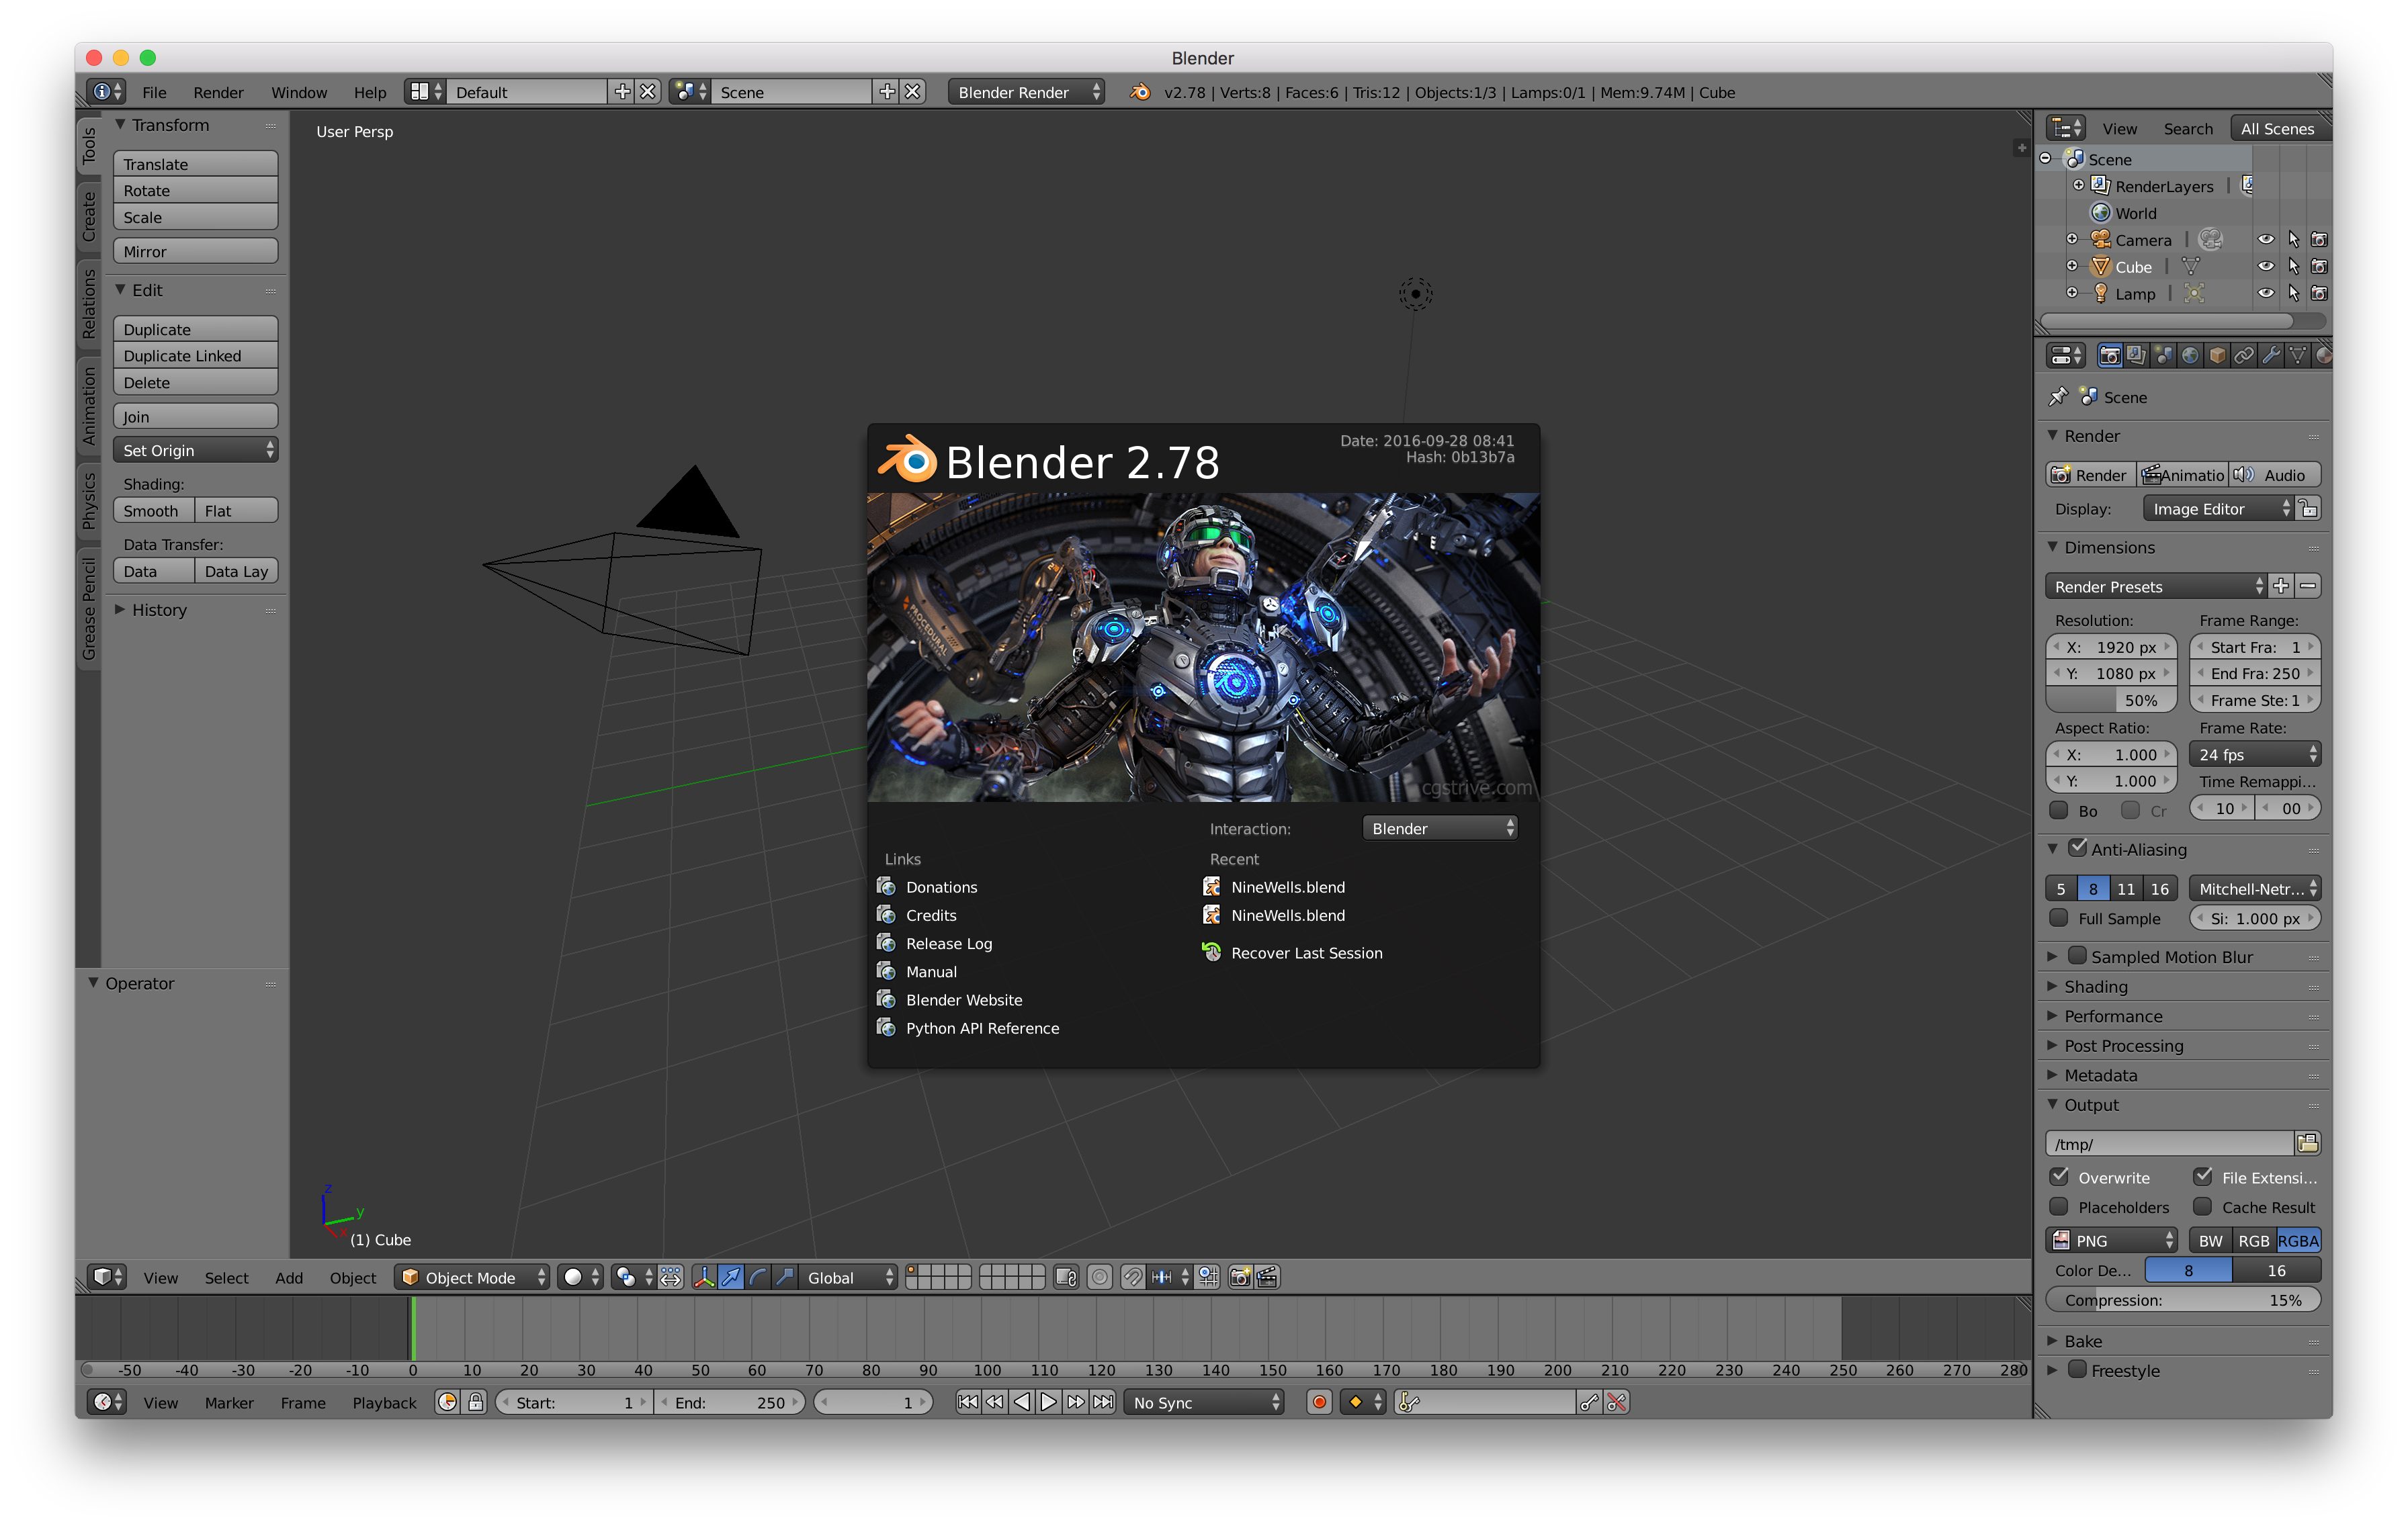
\includegraphics[width=\textwidth]{blender.png}
\end{frame}

\subsection{Bridgeview}

\begin{frame}{Bridgeview}
  Scripts to render visual, semantic and depth images using
  Blender.
  
  \lstinputlisting[language=sh]{sample.sh}
\end{frame}

\begin{frame}{Bridgeview}
  \begin{tikzpicture}
  [var/.style={circle},
  lab/.style={rectangle,draw=mDarkTeal,fill=black!2!white!90!mDarkTeal,
    minimum height=0.8cm,minimum width=1.8cm},
  olab/.style={lab,densely dashed},
  pre/.style={<-,shorten <=1pt,draw},
  post/.style={->,shorten >=1pt,draw}]

%  \clip (1.5,-2.5) rectangle (14.5,4.5);

  \node[lab] (mod) at (0,0) {Model};

  \node[olab] (veg) at (3,0) {Vegetation}
  edge[pre] (mod);

  \node[lab] (pts) at (6,0) {Points}
  edge[pre] (veg);

  \node[lab] (vis) at (8.8,2) {Visual}
  edge[pre,bend right=30] (pts);
  \node[lab] (dep) at (8.8,0) {Depth}
  edge[pre] (pts);
  \node[lab] (sem) at (8.8,-2) {Semantic}
  edge[pre,bend left=30] (pts);

  \node[olab] (mat) at (5,2) {Materials}
  edge[post] (vis);
  \node[olab] (lab) at (5,-2) {Labels}
  edge[post] (sem);
\end{tikzpicture}

\end{frame}

\begin{frame}{TODO}
  Figures!
\end{frame}

\section{Model}

\begin{frame}{Part-based segmentation}
  \begin{description}
  \item[Baseline] U-NET trained on part labels
  \item[Proposed architecture] Hierarchical U-NET --- each decoder
    module outputs a different label (class label, part label,
    geometric label)
  \end{description}
  \begin{figure}[h]\centering
    \vspace{-1cm}
    \def\svgwidth{10cm}
    %% Creator: Inkscape inkscape 0.91, www.inkscape.org
%% PDF/EPS/PS + LaTeX output extension by Johan Engelen, 2010
%% Accompanies image file 'net.eps' (pdf, eps, ps)
%%
%% To include the image in your LaTeX document, write
%%   \input{<filename>.pdf_tex}
%%  instead of
%%   \includegraphics{<filename>.pdf}
%% To scale the image, write
%%   \def\svgwidth{<desired width>}
%%   \input{<filename>.pdf_tex}
%%  instead of
%%   \includegraphics[width=<desired width>]{<filename>.pdf}
%%
%% Images with a different path to the parent latex file can
%% be accessed with the `import' package (which may need to be
%% installed) using
%%   \usepackage{import}
%% in the preamble, and then including the image with
%%   \import{<path to file>}{<filename>.pdf_tex}
%% Alternatively, one can specify
%%   \graphicspath{{<path to file>/}}
%% 
%% For more information, please see info/svg-inkscape on CTAN:
%%   http://tug.ctan.org/tex-archive/info/svg-inkscape
%%
\begingroup%
  \makeatletter%
  \providecommand\color[2][]{%
    \errmessage{(Inkscape) Color is used for the text in Inkscape, but the package 'color.sty' is not loaded}%
    \renewcommand\color[2][]{}%
  }%
  \providecommand\transparent[1]{%
    \errmessage{(Inkscape) Transparency is used (non-zero) for the text in Inkscape, but the package 'transparent.sty' is not loaded}%
    \renewcommand\transparent[1]{}%
  }%
  \providecommand\rotatebox[2]{#2}%
  \ifx\svgwidth\undefined%
    \setlength{\unitlength}{525.37144928bp}%
    \ifx\svgscale\undefined%
      \relax%
    \else%
      \setlength{\unitlength}{\unitlength * \real{\svgscale}}%
    \fi%
  \else%
    \setlength{\unitlength}{\svgwidth}%
  \fi%
  \global\let\svgwidth\undefined%
  \global\let\svgscale\undefined%
  \makeatother%
  \begin{picture}(1,0.37623802)%
    \put(0,0){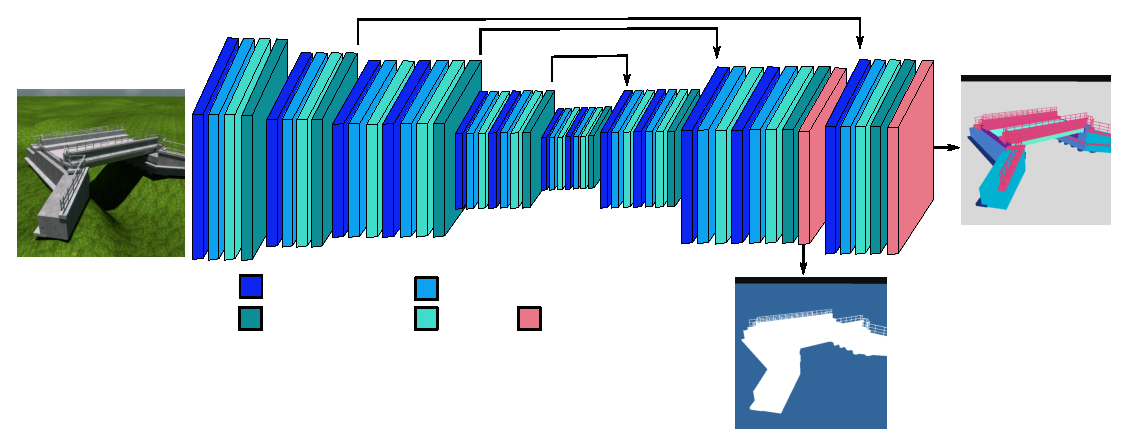
\includegraphics[width=\unitlength]{net.eps}}%
    \put(0.07939957,0.33727883){\color[rgb]{0,0,0}\makebox(0,0)[b]{\smash{RGB image\\ 3 channels}}}%
    \put(0.06036543,0.14204285){\color[rgb]{0,0,0}\makebox(0,0)[lb]{\smash{\textit{Input}}}}%
    \put(0.57647368,0.10701034){\color[rgb]{0,0,0}\makebox(0,0)[lb]{\smash{\textbf{class labels:}\textbf{\\ }   bridge\\    terrain\\    sky}}}%
    \put(0.87864228,0.17372839){\color[rgb]{0,0,0}\makebox(0,0)[lb]{\smash{\textbf{  parts labels:}\textbf{\\ }   deck\\ \textit{      beam}\textit{\\ }   up-deck\\ \textit{      handrail}\textit{\\ }\textit{      kerb}\textit{\\ }   under-deck\\ \textit{      abutment}\textit{\\ }\textit{      wingwall}}}}%
    \put(0.23036758,0.12683161){\color[rgb]{0,0,0}\makebox(0,0)[lb]{\smash{\textit{conv(3x3)}}}}%
    \put(0.39014627,0.09619693){\color[rgb]{0,0,0}\makebox(0,0)[lb]{\smash{\textit{ReLU}}}}%
    \put(0.38993328,0.12311719){\color[rgb]{0,0,0}\makebox(0,0)[lb]{\smash{\textit{batch normalisation}}}}%
    \put(0.2295754,0.09747951){\color[rgb]{0,0,0}\makebox(0,0)[lb]{\smash{\textit{pooling(2x2) }}}}%
    \put(0.48438471,0.09619693){\color[rgb]{0,0,0}\makebox(0,0)[lb]{\smash{\textit{SoftMax}}}}%
  \end{picture}%
\endgroup%

    \vspace{-0.5cm}
  \end{figure}
\end{frame}
\note{We propose a dedicated architecture for part-based segmentation,
  where the network predicts different labels at each level. The
  network first has to recognise if the pixel belongs to the bridge
  class or other class (e.g.\ vegetation, terrain), and then recognise
  the part and the geometric shape.  Experiments show that this
  approach is better than just predicting directly only the part. In
  the hierarchical case we inject more supervision, hence results are
  better.}

\section{Results}

\begin{frame}{Results}
  \begin{block}{Experiments}
    \begin{enumerate}
    \item RGB vs RGB-D using the baseline architecture
    \item Flat vs hierarchical using RGB-D input
    \end{enumerate}
  \end{block}
  \begin{block}{Evaluation}
    \begin{description}
    \item[Global avg.\ accuracy] among all the pixels, how many have
      been labelled correctly on average per image
    \item[Per class avg.\ accuracy] how many pixels have been labelled
      correctly for each class on average
    \end{description}
  \end{block}
\end{frame}
\note{Two sets of experiments:\@ RGB vs.\ RGB-D: to see if adding
  depth helps or if appearance is enough for classification; flat vs
  hierarchical: to prove that the different levels of supervision are
  improving the performance. For quantitative evaluation, we use two
  measures.}

\begin{frame}{Quantitative results}
  \begin{tabular}{lll}
    \toprule
    Architecture/input & Global accuracy & Per class accuracy \\
    \midrule
    RGB baseline & $93.4072$ & $20.64704$ \\
    RGB+D baseline & $95.0932$ & $22.63335$ \\
    RGB+D hierarchical & $96.59791$ & $28.53001$ \\
    \bottomrule
  \end{tabular}
\end{frame}
\note{The quantitative results show that adding depth helps over RGB
  alone. This is because depth tends to have less variety, it is more
  reliable compared to texture, and also RGB can be more influenced by
  shadows, noise.}
\note{The hierarchical training improves significantly the results.
  It can be noted that although the global accuracy is very high, the
  per class accuracy is very low. This is because there are a few very
  small and rare classes (like bearings) which have (as expected) a
  very low accuracy, bringing the overall average accuracy to a low
  level.}

\begin{frame}{Qualitative results: hierarchical U-NET with RGB+D as
    input}
  \begin{figure}[h]\centering
    \only<1>{
      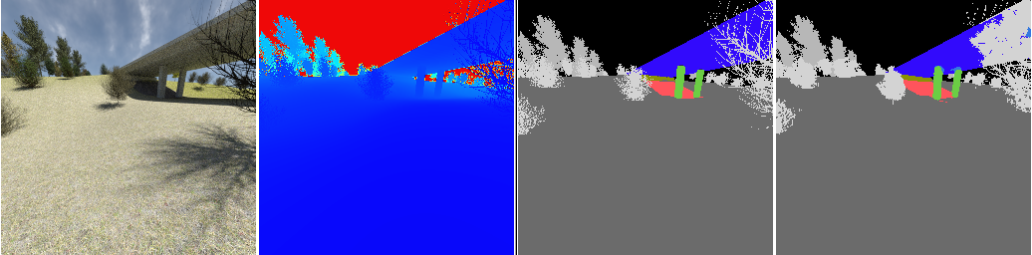
\includegraphics[width=10cm]{ex1.png}
      \vspace{1em}
      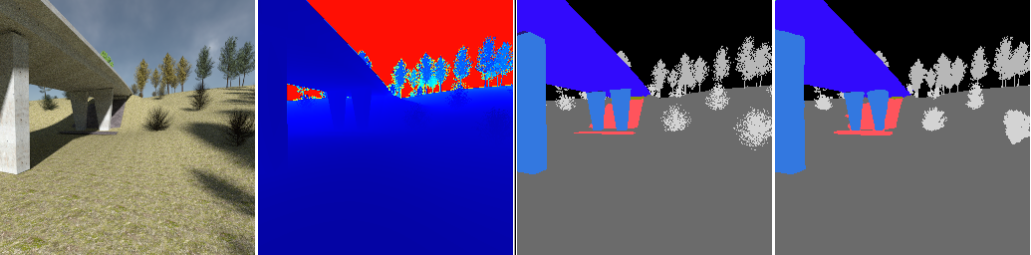
\includegraphics[width=10cm]{ex2.png}
    }
    \only<2>{
      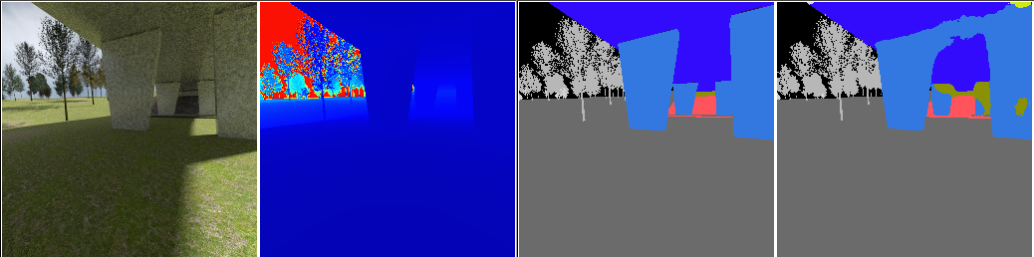
\includegraphics[width=10cm]{ex3.png}
      \vspace{1em}
      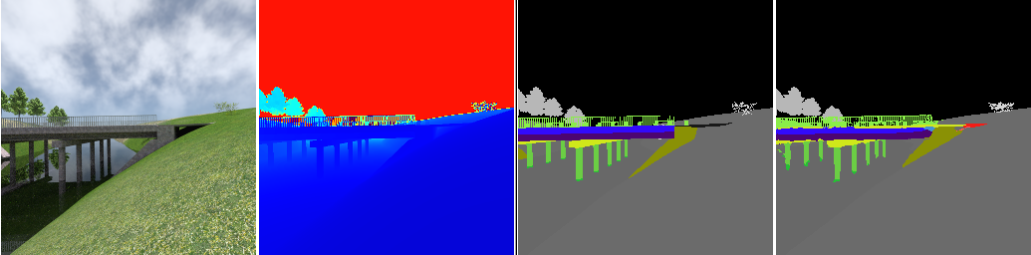
\includegraphics[width=10cm]{ex4.png}
    }
    \only<3>{
      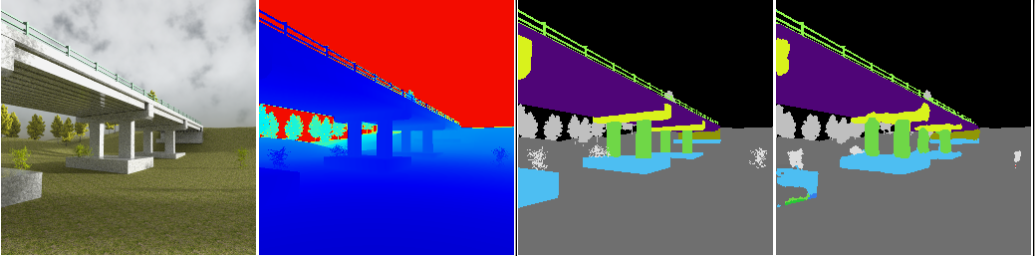
\includegraphics[width=10cm]{ex5.png}
      \vspace{1em}
      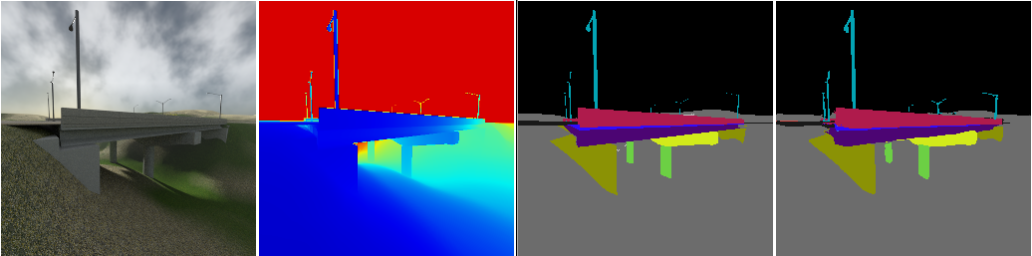
\includegraphics[width=10cm]{ex6.png}
    }
  \end{figure}
\end{frame}
\note{Qualitative results on test images (images that were not used
  during training):\@ The accuracy is very good at the class level,
  terrain, vegetation, bridge are very well recognised. The main
  parts of the bridge are also well identified: columns, piers,
  abutment, deck.}
\note{There are of course mistakes as well, like in the picture on
  top, the network unifies the two piers.  But overall it does get the
  classes, even the smaller ones like handrails.}
\note{\ldots and light-poles. There is a lot of potential in this
  approach. The challenge now is to get some real labelled data, to
  fine-tune the network on real data, so that it is capable of
  segmenting any real image of a bridge.}

\section{Conclusion}

\begin{frame}{Summary}
  Data generation scripts are open source (GPL) and available from

  \begin{center}
    \href{https://github.com/jaantoots/bridgeview}{github.com/jaantoots/bridgeview}
  \end{center}

  Model files and the complete dataset will be made available.
\end{frame}

\begin{frame}[standout]
  Questions?
\end{frame}

\end{document}
